\subsection{\uavs (\vants) }

\vants são definidos por \cite{uav_roadmap2005} como veículos aéreos que não carregam operadores humanos que são capazes de voar autonomamente ou serem pilotados remotamente e não são limitados por restrições humanas. Pelo fato de não carregarem pilotos, estes tipos de aeronaves podem ser sujeitos aos mais variados tipos de aplicação.
Exemplos básicos são áreas de baixo oxigênio, áreas contaminadas por resíduos tóxicos ou produtos químicos nocivos à saúde humana.

Estes veículos recentemente alcançaram um crescimento não previsto e diversas aplicações em áreas civis e militares têm sido desenvolvidas nos mais diversos domínios \cite{Valavanis2007}.


Atualmente existe uma grande diversidade de modelos de VANTs. Podendo variar em vários tamanhos, formatos, configurações e propósito.
Determinados \vants variam de aeronaves do tamanho de insetos à \vants com porte relativo a aviões comerciais \cite{Bone2003}.

Não se considerando apenas aspectos como segurança, mas também aspectos como extensão, \vants de vários tamanhos e modelos podem ser utilizados para monitoramento em recuperação de desastres, detecção de eventos, ente outros. 

Em aplicações militares, \vants trabalham por meio de execução de missões que não necessitam do uso de pilotos \cite{Bone2003}. Essas missões são classificadas como 3-D.


Em \cite{uav_roadmap2005} 3-D são definidas como:
\begin{description}
\item[\emph{Dull} - Tedioso: ]
\vants podem realizar missões consideradas tediosas para pilotos. Como exemplo a viagem rotineira de um vôo de 30 horas realizada por uma equipe do exército americano de Missouri até a Sérvia por 34 dias no conflito de Kosovo em 1999 \cite{uav_roadmap2005}. 

\item[\emph{Dirty} - Sujo: ]
Casos em que se torna necessário o monitoramento de alguma região contaminada. Entre 1946 e 1948, a força aérea (\emph{The Air Force}) e a marinha (\emph{The Navy}) americanos utilizaram \vants para recolherem amostras radioativas após detonação de bombas nucleares \cite{uav_roadmap2005}.

\item[\emph{Dangerous} - Perigoso: ]
Missões de exploração ou reconhecimento podem apresentar riscos aos pilotos. Segundo \cite{uav_roadmap2005}, 25\%  dos pilotos dos grupos de reconhecimento do exército americano foram perdidos durante a Segunda Guerra Mundial no norte da África, enquanto somente 5\% dos pilotos de bombardeiros foram perdidos sobrevoando a Alemanha.

\end{description}

O restante dessa sessão apresenta, de forma resumida, os avanços e pesquisa em VANTs. Na próxima subsessão serão apresentados os modelos básicos de \vants.

\subsubsection{Modelos e Arquiteturas de \vants}

Esta seção apresenta, de forma condensada, os avanços das pesquisas em modelos e arquiteturas de Veículos Aéreos Não Tripulados. Serão apresentados os principais modelos de \vants utilizados atualmente. Destaca-se o desenvolvimento de aeronaves direcionadas ao uso em aplicações militares.

Os principais modelos de \vants da atualidade foram projetados primeiramente com propósito de missões de reconhecimento e vigilância. Porém, esforços têm sido realizados para o desenvolvimento de \vants que representem maior representatividade em campos de batalha, como detectar alvos aéreos, monitorar movimento de tropas inimigas à auxílio de artilharia em batalhas \cite{Bone2003}.

A Tabela ~\ref{tbl:categorization} apresenta as categorias de \vants reconhecidas pelos especialistas no assunto. Porém, por não ser objetivo deste trabalho realizar uma investigação detalhada a respeito dos modelos de \vants, será adotada a convenção proposta por \cite{Drew2005} para que o assunto não se extenda demasiadamente.
\begin{table}[h!]
\centering
\small
	\begin{tabular}{|p{3.0cm}| c c  c c c| }
		\hline
		Categoria&Alcance&Altitude&Autonomia&P.M.D.\footnotemark[1]&Atividade\\
		  	      & (km)         &   (km)     &(horas) & (kg)    & \\
		\hline
		\multicolumn{6} {| l |}{Táticos} \\
		\hline
		Nano& < 1 &100 &< 1 &< 0,025& sim \\
		Micro& < 10 &250 &1 &< 5 &sim \\
		Mini &< 10 &150 a 300& < 2& < 30& sim \\
		Close Range &10 a 30& 3.000& 2 a 4 &150& sim \\
		Short Range &30 a 70 &3.000 &3 a 6 &200 &sim \\
		Medium Range & 70 a 200 &5.000 &6 a 10 &1.250 &sim \\
		Medium Range Endurance  &> 500 &8.000 &10 a 18 &1.250& sim \\
		Low Altitude Deep Penetration &> 250 &50 a 9.000 &0,5 to 1 &350 &sim \\
		Low Altitude Long Endurance  &> 500 &3.000 &> 24 &< 30 &sim \\
		Medium Altitude Long Endurance &> 500 &14.000 &24 a 48 &1.500 &sim \\
		\hline

		\multicolumn{6} {| l |}{Estratégicos} \\
		\hline
		High Altitude Long Endurance & > 2000& 20.000 &24 a 48& 12.000& sim \\
		\hline
%
%		\multicolumn{6} {| l |}{Propósito Especial} \\
%		\hline
%		Unmanned Combat Aerial Vehicle & approx. 1500&10.000& approx. 2& 10.000& sim \\
%		Lethal & 300 & 4.000& 3 a 4 &250& sim \\
%		Decoy  &0 a 500 &5.000 &< 4 &250 &sim \\
%		Stratospheric & > 2000 &20.000 a 30.000 &> 48 &TBD\footnote{\emph{To Be Defined} - A Definir} &não \\
%		Exo-stratospheric & TBD &> 30.000 &TBD& TBD& não\\
%		Space  &TBD &TBD &TBD& TBD& não\\
%		\hline
	\end{tabular}
	
	\caption{Categorias de \vants.}
	\label{tbl:categorization}
\end{table}



\cite{Drew2005} dividem os \vants em duas principais classes baseadas na extensão das aeronaves. Neste trabalho serão consideradas como Grande Porte e Pequeno Porte (Micro, Portáteis e Multi-missões).

%O foco deste trabalho não é uma investigação sobre os modelos e arquiteturas de \vants. Portanto,  neste tópico serão apresentados, de forma resumida, alguns modelos comuns de UAVs. Mais informações sobre arquiteturas de \vants podem ser encontradas em \cite{Drew2005,uav_roadmap2005, Bone2003,Holder2001}.

\footnotetext[1]{Peso Máximo de Decolagem - É o peso máximo permitido para que um avião consiga realizar vôos em plena capacidade. }
\addtocounter{footnote}{1}

\paragraph{\vants de Grande Porte:}
Segundo \cite{Drew2005}, \vants de grande porte têm sistemas de lançamento e recuperação que podem ser separados dos seus sistemas de controle e exploração de dados. Os VANTs apresentam mecanismos que podem ser controlados separadamente, como por exemplo, coleta das informações e comunicação via satélite.



 \subparagraph{\emph{Global Hawk}: }

 É o \vant mais caro já produzido. Este \vant é capaz de alcançar altitudes elevadas (65.000 pés\footnote{A medida de 1 pé é de aproximadamente 30cm.}), e longos períodos de ativididade de 28 a 32 horas. Este modelo é capaz de prover imagens próximas a tempo real em grandes áreas geográficas (cerca de 40.000 nm\footnote{Milhas náuticas quadradas. 1 milha náutica representa 1,828 km.} por dia) \cite{uav_roadmap2005}.

Segundo \cite{Drew2005}, o \emph{Global Hawk} foi o primeiro \vant a realizar uma viagem trans-pacífico, quando voou da Califórnia à Austrália de 22 a 23 de Abril de 2001.

O preço de um \emph{Global Hawk} completo é próximo de 54 milhões de dólares e o preço de cada estação terrestre para controle
é de 16 milhões.

\begin{figure}[h!]
\centering
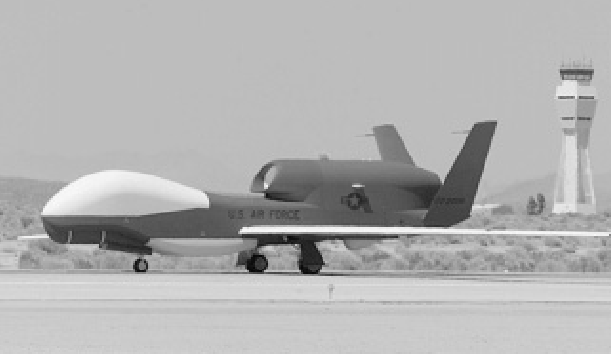
\includegraphics[width=10cm]{pictures/global_hawk.png}
\caption{Global Hawk}
 \label{fig:global_hawk}
\end{figure}


Este modelo apresenta 13,5 metros de extensão, peso de 12.144 quilos e possui o tamanho comparável ao de um jato comercial de médio porte \cite{Drew2005,uav_roadmap2005,Bone2003}.


\subparagraph{ \emph{Predator}: }

 O modelo \emph{Predator} é um \vant  de grande porte, considerado de média a alta altitude (15.000 a 25.000 pés), apresenta 
uma extensão de aproximadamente 11 metros,  4.767 quilos de peso e autonomia de vôo de 16 a 30 horas.

\begin{figure}[h!]
\centering
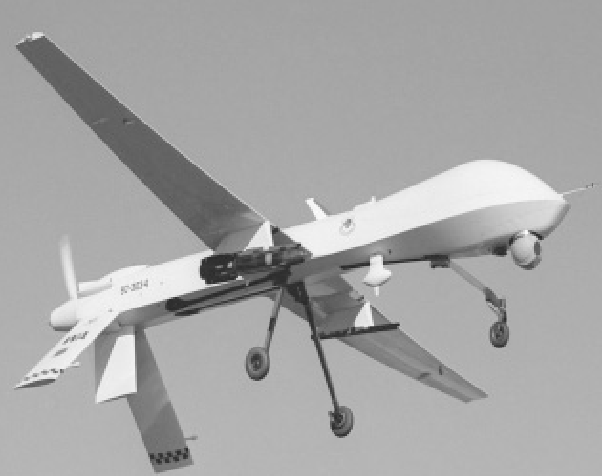
\includegraphics[width=10cm]{pictures/predator.png}
\caption{Predator}
 \label{fig:predator}
\end{figure}

A primeiro propósito deste modelo de \vant é atuar como vigilante em uma determinada área de interesse. Este \vant é equipado com uma variedade de sensores para capturar imagens de alta resolução em determinadas áreas.
O segundo propósito para o desenvolvimento deste modelo de aeronave é atuar em conjunto de inteligente de \uavs. 

Cada \emph{Predator} tem um custo aproximado de 4.5 milhões de dólares. Um sistema completo de \emph{Predator}s custa em média 30 milhões de dólares \cite{Drew2005,uav_roadmap2005,Bone2003}.



\paragraph{\vants de Pequeno Porte}

Em \cite{Drew2005}, \vants de Pequeno Porte são divididos nas seguintes subclasses:

\begin{description}

\item[Micro-\vants: ]
São aeronaves de menor porte e geralmente são utilizadas para missões de reconhecimento, pois seu tamanho reduzido permite uma grande versatilidade. Uma característica importante é que estes modelos são indicados somente para operações durante o dia e com boas condições climáticas, visto que as restrições de tamanho dificultam a locomoção em más condições climáticas. Estes modelos são projetados para carregarem cargas de peso inferior a 200g.

\item[Portáteis: ]
São modelos direcionados à aplicações de pequenos times de \vants. Esses modelos se adaptam bem à aplicações colaborativas. Podem ser carregados e lançados por uma pessoa. Geralmente estes \vants apresentam autonomia de vôo de aproximadamente 1 a 2 horas, e normalmente carregam cargas de até 25 kg.

\item[Multi-Missão: ]
Conhecidos como \vants  de propósito geral, estes são os maiores entre os menores modelos de \vants e geralmente apresentam autonomia de voo de 10 a 12 horas e possuem capacidade para carregar cargas de 25 a 110 kg. Estes \vants são projetados para missões operacionais variadas, sendo considerados as aeronaves mais versáteis da categoria. Exemplos comuns de aplicações são: carregamento de suprimentos para o campo de batalha, distribuição (\emph{deployment}) de sensores em uma região, monitoramento, entre outros.

\end{description}


\subparagraph{\emph{RAVEN}:}
É um \vant portátil que carrega câmeras infra-vermelho frontais e laterais. Este modelo pode ser pilotado remotamente ou através de vôo autônomo baseado em GPS. Em muitos casos 
este modelo é utilizado para missões de reconhecimento e vigilância, destacando-se no uso para reconhecimento noturno devido o uso de suas câmeras infra-vermelhas.

Este modelo pode sobrevoar altitudes de no máximo 14.000 pés, porém seus usos mais comuns são em missões variando de 150 a 500 pés de altura. Possui um raio de alcance de 
13 a 18,5 km e autonomia de 60 a 90 minutos, alcançando velocidade máxima de 110 km/h e velocidade de cruzeiro de aproximadamente 50 km/h \cite{uas_2009}. 

A instalação de um sistema composto por dois \emph{RAVENs} custa aproximadamente 139.000 dólares \cite{Drew2005}. 

Na Figura ~\ref{fig:raven} pode ser vista a operação de lançamento de um \vant do tipo \emph{RAVEN}.

\begin{figure}[h!]
\centering
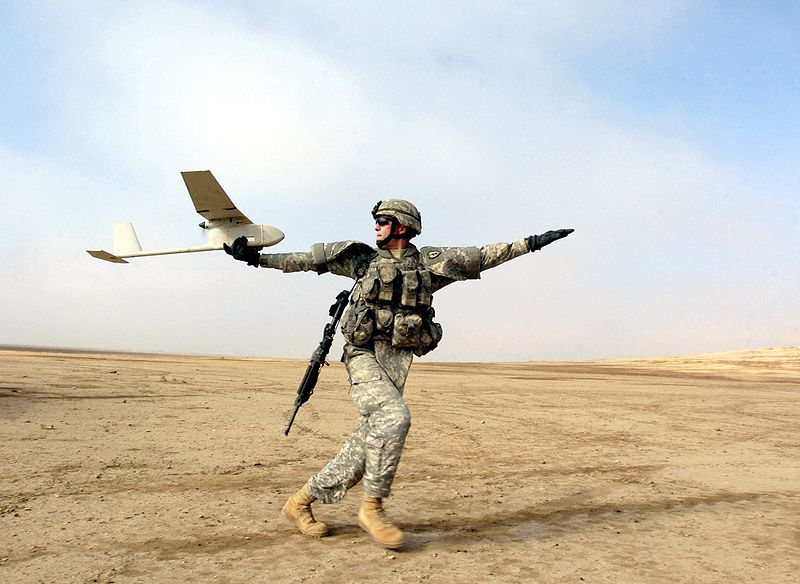
\includegraphics[width=10cm]{pictures/launching_raven.jpg}
\caption{Soldado americano lançando um \emph{RAVEN} }
 \label{fig:raven}
\end{figure}




\subparagraph{ \emph{Pointer}:}
Este \vant  portátil foi desenvolvido para prover dados em tempo real em uma grande variedade de aplicações. Sua missão primária é a de reconhecimento e vigilância de áreas
utilizando sensores EO\footnote{Sensor Eletro-Óptico.} e IR\footnote{Infra-red, em português: Infra-Vermelho.}, bem como sensores de detecção química. Este modelo apresenta comprimento de asa de 9 pés e pesa apenas 3,7 kg. Um \emph{Pointer} tem autonomia de vôo de aproximadamente 2 horas e pode alcançar altitudes de até 500 pés carregando cargas de no máximo 500g \cite{uas_2009}. Um sistema de dois \emph{Pointers} custa aproximadamente 133.000 dólares \cite{Bone2003}. 

Na Figura ~\ref{fig:launching_pointer} pode ser visto o lançamento de um \emph{Pointer}. 

\begin{figure}[h!]
\centering
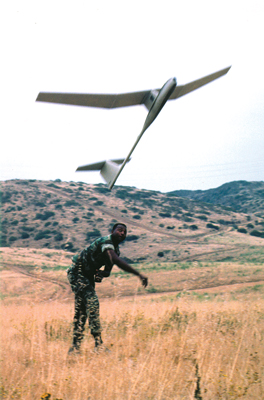
\includegraphics[width=6cm]{pictures/launching_pointer.jpg}
\caption{Lançamento de um \emph{Pointer} }
 \label{fig:launching_pointer}
\end{figure}


\subparagraph{ \emph{BATCAM}:}
O \emph{The Battlefield Air Targeting Camera Micro Air
Vehicle} (BATCAM) é um modelo altamente avançado de Micro-VANT. Esse \vant  é menor que outros modelos como \emph{Pointer}, \emph{Raven} e \emph{FPASS}.
O \emph{BATCAM} tem um peso de aproximadamente700g, apresenta uma autonomia de vôo de apenas 30 minutos, altitude de vôo de 500 pés e uma capacidade de carga de
apenas 200g. Este modelo foi construído para missões de reconhecimento e carrega sensores IR e EO.



Devido o seu tamanho reduzido. Este modelo pode ser utilizado em diversos tipos de operação, como infiltração, monitoramento e vigilância \cite{Drew2005}. 

\begin{figure}[h!]
\centering
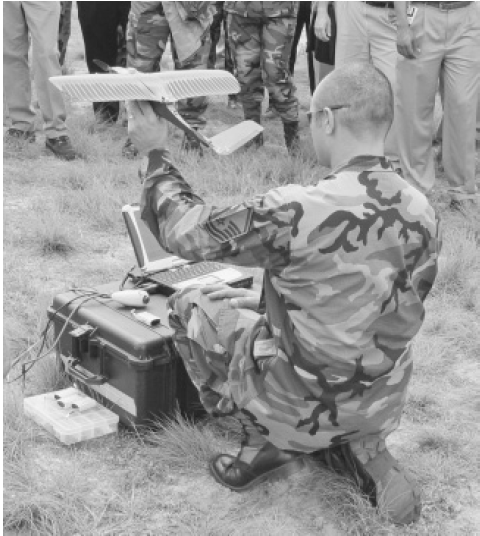
\includegraphics[width=10cm]{pictures/batcam_system.png}
\caption{ Soldado operando um \emph{BATCAM} }
 \label{fig:holding_batcam}
\end{figure}

Na Figura ~\ref{fig:holding_batcam} é apresentado um sistema \emph{BATCAM}.



\subparagraph{ \emph{Dragon Eye}:}
O \vant \emph{Dragon Eye} foi projetado para missões de reconhecimento, vigilância e detecção de alvos. Com um comprimento de asa de apenas 18 cm e peso de 2,5 kg, este modelo pode ser carregado ate mesmo em uma mochila e ser lançado facilmente em diversos tipos de situação.

Este modelo pode voar em velocidades de aproximadamente 75 km/h, cobrindo uma área de até 10km e retornando em 1 hora. Geralmente alcança altitudes de 300 a 500 pés.
Devido a sua grande versatilidade, este \vant tem sido utilizado em diversas aplicações urbanas \cite{Drew2005,uav_roadmap2005}.

Um sistema \emph{Dragon Eye} é composto por 2 veículos aéreos, 4 câmeras, 2 frentes removíveis e uma estação terrestre de controle. O custo de um sistema \emph{Dragon Eye} é
de aproximadamente 65.000 dólares. Na Figura ~\ref{fig:dragon_eye} pode ser visto um sistema \emph{Dragon Eye}.

\begin{figure}[h!]
\centering
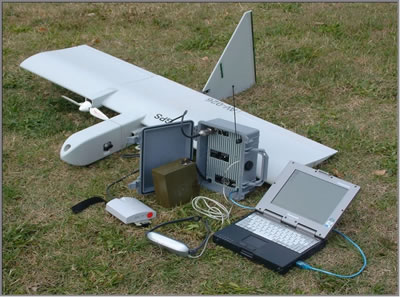
\includegraphics[width=10cm]{pictures/dragon_eye_system.jpg}
\caption{Sistema \emph{Dragon Eye} }
 \label{fig:dragon_eye}
\end{figure}


\subsubsection{Aplicações utilizando \vants}
Atualmente, a pesquisa em \vants tem se concentrado fortemente em aplicações militares, variando de aplicações de monitoramento, vigilância, suporte de ataque aéreo, entre outros. Atualmente, segundo \cite{Valavanis2007} a pesquisa em diferentes tipos de aplicação (não somente militares) tem crescido e ampliado os horizontes de desenvolvimento.

Na Tabela~\ref{tbl:vants_por_ano} é possível visualizar o desenvolvimento das aplicações utilizando \vants nos últimos anos \cite{Bryner2007}. Bem como na Figura~\ref{fig:qt_uav_app} podem ser visualizadas as quantidades de \vants utilizadas nos diferentes tipos de aplicações \cite{Bryner2007}. Pode-se notar um aumento significativo no número de aplicações comerciais e de propósito geral nos anos de 2008 e 2009.


\begin{table}[h!]
\centering
	\begin{tabular}{| l | c | c | c | c | c | c |}
		\hline
		Aplicações/Ano & 2004 & 2005 & 2006 & 2007 & 2008 & 2009 \\
		\cline{2-7}
		 & Qt & Qt & Qt & Qt & Qt & Qt  \\
		\hline
		Civil/Comercial  & 33 &  55  & 47  & 61  & 115  & 150 \\
		%\hline
		Militar  & 362  & 397  & 413  & 491  & 578  & 683 \\
		%\hline
		Propósito Geral &  39  & 44  & 77  & 117  & 242  & 260 \\
		%\hline
		Pesquisa  & 43  & 35  & 31  & 46  & 54  & 66 \\
		%\hline
		Desenvolvimento de \vants &   & 219  & 217  & 269  & 293  & 329 \\
		\hline
	\end{tabular}

	\caption{Aplicações de \vants por ano.}
	\label{tbl:vants_por_ano}
\end{table}



\begin{figure}[h!]
\centering
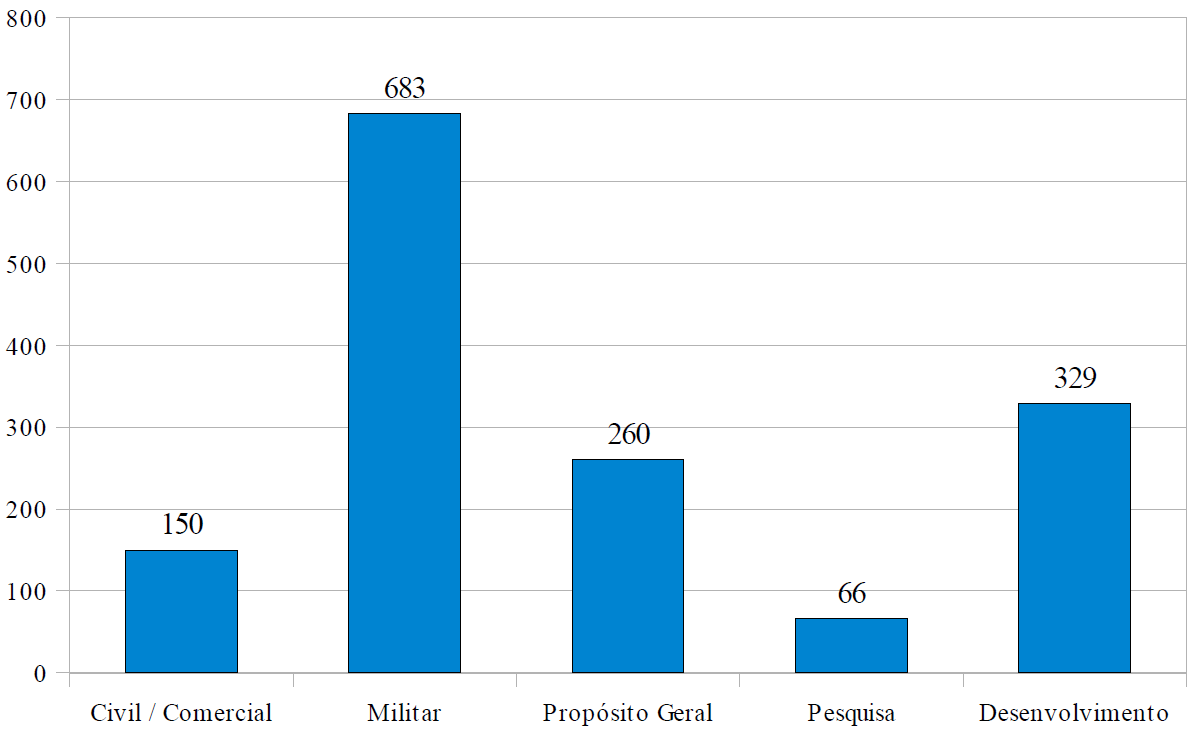
\includegraphics[width=13cm]{pictures/qt_uavs_app.png}
\caption{Quantidade de \vants por classe de aplicação. }
 \label{fig:qt_uav_app}
\end{figure}



\subsubsection{Desenvolvimento de \vants}

Diversas nações têm se destacado quanto ao desenvolvimento de VANTs. Os Estados Unidos é o país que atualmente possui mais aeronaves produzidas (386), e representa 32,44\% da
produção mundial de aeronaves não tripuladas. Outras nações como Israel (83 - 6,97\%),  França (77 unidades - 6,47\%), Rússia (59 unidades - 4,96\%) e Reino Unido (65 - 5,46\%) também têm apresentado resultados significativos quanto ao número de \vants produzidos. O Brasil, ainda iniciando suas pesquisa em \vants, possui 6 unidades produzidas, contabilizando apenas 0,5\% das aeronaves não tripuladas produzidas no mundo.

Na Tabela~\ref{tbl:country} encontram-se os dados resumidos do desenvolvimento de \vants em âmbito mundial \cite{Bryner2007}.

\begin{table}[h!]
\centering
	\begin{tabular}{| l | c | c |}
		\hline
		País & Número de Aeronaves & \% \\
		\hline
		EUA & 386 & 32,44 \\
		Israel & 83 & 6,97 \\
		França & 77 & 6,47 \\
		Reino Unido & 65 & 5,46 \\
		Iran & 38 & 3,19 \\
		Brasil & 6 & 0,50\\
		Outros Países & 535 & 44,97 \\
		\hline
	\end{tabular}

	\caption{Desenvolvimento de \vants por nação.}
	\label{tbl:country}
\end{table}


\subsubsection{Pesquisas em \vants}
Diversos esforços têm sido realizados nas pesquisas sobre VANTs, bem como diversas aplicações têm sido desenvolvidas. Este tópico apresentará alguns avanços da pesquisa e
utilização prática de \vants em diversos cenários.

\begin{description}

\item[Exploração em Regiões Polares: ]
\cite{Storvold2009} mostra em \emph{Scientific UAS Missions in the Polar Regions} alguns avanços do uso de \vants em aplicações de exploração e monitoramento de regiões polares. A utilização de aeronaves não tripuladas neste tipo de missão se justifica pelo fato das limitações de resoluções espaciais e temporais dos satélites que cobrem estas áreas. O uso de \vants proporciona medidas mais precisas pelo fato de serem realizadas com mais proximidade. Outro fator destacado na utilização de \vants para este tipo de exploração é que a utilização de
aeronaves pilotadas por humanos neste tipo de região se apresenta altamente custoso e perigoso devido as condições climáticas desfavoráveis da região. A utilização de \vants proporcionou redução dos gastos e melhorou a acurácia das medidas na região. 

\item[Recuperação de Desastres e Incêndios: ]
Uma grande variedade de organizações (além das organizações militares), ultimamente, tem considerado o uso de \vants  numa grande variedade de aplicações. O grupo de bombeiros
WMFS (\emph{West Midlands Fire Service}), do Reino Unido, tem utilizado o sistema \emph{ISiS} para a suporte em casos de desastres. \cite{Mika2009} relata casos de uso do sistema \emph{ISiS} para suporte em diversos desastres. A utilização de câmeras de alta resolução instaladas em \vants de pequeno porte permite que os bombeiros visualizem a situação e provê suporte para que sejam tomadas decisões mais coerentes com cada caso.

\begin{figure}[h!]
\centering
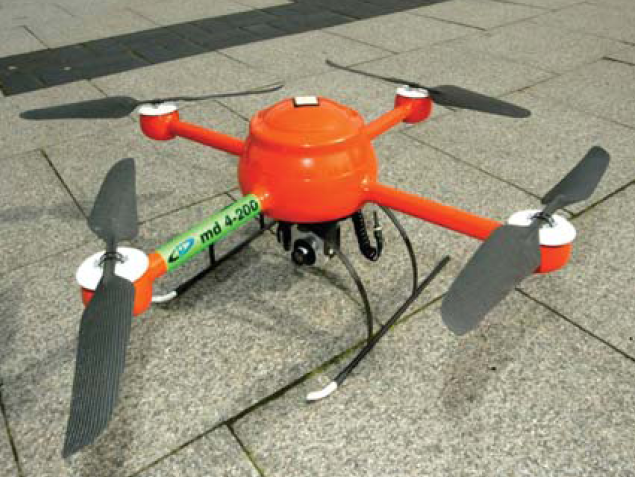
\includegraphics[width=10cm]{pictures/mq4200.png}
\caption{ \emph{MD4-200}: \vant utilizado por \emph{West Midlands Fire Service} para reconhecimento em locais de desastre. }
 \label{fig:md4-200}
\end{figure}

O \vant utilizado nas missões do WMFS é conhecido como MD4-200. Este \vant é composto predominantente de fibra de carbono e plástico reforçado. Tem um peso de 900g e apresenta três principais sensores: Câmera de vídeo de alta resolução, câmera fotográfica de alta resolução (12 mega pixels) e um sensor infra-vermelho. Este modelo também possui alcance de 3km a partir da estação base. Na figura~\ref{fig:md4-200} pode ser visualizado um MD4-200 utilizado nas operações citadas.

Por volta de 20\% dos terremotos de larga escala ocorrem no Japão, e também 7\% dos vulcões em atividade estão localizados neste país. Danos por tempestades, inundações e nevascas também têm sido comuns neste território. \cite{Sasa2008} demonstram os avanços nas pesquisas do \emph{JAXA Aviation Program Group} e propõem soluções para a melhoria da infraestrutura de previsão de desastres japonesa.

\item[Controle Autônomo: ]
Em \cite{Semsch2009} são tratados problemas de controle autônomo de \vants. Neste trabalho os autores apresentam problemas em que se necessita controlar um time de vários \vants para que se promova vigilância em ambientes urbanos complexos. São demonstrados problemas complexos como monitorar áreas de difícil visualização, como regiões com prédios altos e ruas estreitas. Outros autores como \cite{KimAndKim} e \cite{Sarmiento2004} também trabalharam problemas de controle autônomo e oclusão.

\item[ Sistemas para evitar colisão (\emph{Collision Avoidance}):]
Diversos esforços têm sido gastos no desenvolvimento de sistemas para se evitar colisão em grupos de \vants (\emph{Collsion Avoidance}). Tratam-se de casos onde se torna necessário controlar grupos de \vants (ou apenas um único) para que os mesmos não colidam entre si, ou colidam com algum obstáculo.

Segundo \cite{Hutchings2007}, sistemas de \emph{Collision Avoidance} ou \emph{Sensing Avoidance} são divididos em:
	\begin{description}
		\item[S\&A estratégico: ]  Conflitos potenciais são detectados a longo prazo. Isto permite que a rota seja reprogramada e o objeto de conflito possa ser evitado.
		\item[Avisos de Resolução de Conflitos: ] Algum agente externo envia um aviso para que o \vant altere sua rota. O \vant deve esperar e aceitar avisos constantemente.
		\item[Controle Autônomo de S\&A: ] O \vant realiza uma manobra num tempo mínimo de segurança para se evitar a colisão.
	\end{description}

Trabalhos relacionados podem ser encontrados em \cite{Hutchings2007,Bryner2007,Deschenes2004,Taylor2005}, entre outros.

\end{description}

Nesta seção foram apresentados brevemente a motivação, os tipos e modelos de \vants, bem como algumas informações a respeito do desenvolvimento, pesquisas e investimentos nesta área. Muitos outros trabalhos e aplicações de \vants podem ser encontrados e demonstrados. Porém, não é foco deste trabalho fazer um levantamento completo do estado da arte de \uavs. 